\documentclass[conference]{IEEEtran}
\usepackage{cite}
\usepackage{amsmath,amssymb,amsfonts}
\usepackage{graphicx}
\usepackage{float}
\usepackage{url}
\usepackage[hidelinks]{hyperref}
\usepackage{textcomp}
\usepackage{booktabs}
\usepackage{siunitx}
\graphicspath{{source/extracted_images/}}

\begin{document}

\title{Non-Linear Control of a 2-DOF Robotic Arm: Complete Design, Simulation, and Hardware Implementation}

\author{
\IEEEauthorblockN{Ahmed Mostafa}
\IEEEauthorblockA{\textit{Dept. of Mechatronics Engineering} \\
\textit{German University in Cairo (GUC)}\\
Cairo, Egypt}
\and
\IEEEauthorblockN{Andrew Khalil}
\IEEEauthorblockA{\textit{Dept. of Mechatronics Engineering} \\
\textit{German University in Cairo (GUC)}\\
Cairo, Egypt}
\and
\IEEEauthorblockN{Hazim Ashraf}
\IEEEauthorblockA{\textit{Dept. of Mechatronics Engineering} \\
\textit{German University in Cairo (GUC)}\\
Cairo, Egypt}
\and
\IEEEauthorblockN{Mazen Amr}
\IEEEauthorblockA{\textit{Dept. of Mechatronics Engineering} \\
\textit{German University in Cairo (GUC)}\\
Cairo, Egypt}
\and
\IEEEauthorblockN{Samir Sameh}
\IEEEauthorblockA{\textit{Dept. of Mechatronics Engineering} \\
\textit{German University in Cairo (GUC)}\\
Cairo, Egypt}
\and
\IEEEauthorblockN{Youssef Youssry}
\IEEEauthorblockA{\textit{Dept. of Mechatronics Engineering} \\
\textit{German University in Cairo (GUC)}\\
Cairo, Egypt}
}

\maketitle

\begin{abstract}
This paper presents the complete design, simulation, and hardware implementation of a non-linear controlled two-degree-of-freedom (2-DOF) planar robotic arm. The work encompasses mathematical modeling using the Euler--Lagrange formulation, non-linear stability analysis via Lyapunov methods, feedback linearization control synthesis, MATLAB/Simulink simulation validation, and real-time embedded implementation on an Arduino microcontroller. The system employs two 25GA370 DC gear motors with integrated quadrature encoders, 3D-printed PLA+ structural links designed in SolidWorks, and an L298N dual H-bridge motor driver. The feedback linearization controller decouples the highly non-linear joint dynamics, achieving accurate trajectory tracking across the workspace. Simulation results demonstrate convergent position regulation with less than 0.01\,rad steady-state error and circular trajectory tracking with phase error below 0.02\,rad. Hardware validation on the physical prototype confirms the practical feasibility of the non-linear control approach for low-cost educational robotic platforms.
\end{abstract}

\begin{IEEEkeywords}
Non-linear control, robotic manipulator, feedback linearization, Euler--Lagrange, DC motors, embedded systems, MATLAB/Simulink, Arduino, trajectory tracking, Lyapunov stability.
\end{IEEEkeywords}

\section{Introduction}
\label{sec:introduction}

Robotic manipulators are indispensable across modern applications including industrial automation, precision manufacturing, medical surgery, and research~\cite{slotine1991}. Achieving accurate trajectory tracking requires control algorithms that compensate for model uncertainties, disturbances, and the inherent non-linear coupling between joints.

Manipulators are fundamentally multi-input multi-output (MIMO) systems: each actuator influences the motion of multiple links through configuration-dependent inertia, Coriolis/centrifugal coupling, and gravitational effects. These properties render linear control approaches---such as independent PID loops---inadequate for high-performance operation, especially at moderate to high speeds~\cite{spong2020}.

Feedback linearization (also called computed-torque control) addresses this by using the system's known dynamics to construct a control law that exactly cancels the non-linear effects, producing a linearized closed-loop system amenable to classical design techniques~\cite{slotine1991,siciliano2009}.

This paper presents the complete engineering workflow for a 2-DOF planar robotic arm:
\begin{enumerate}
\item Mathematical modeling using Euler--Lagrange dynamics (Section~\ref{sec:modeling}).
\item Feedback linearization controller design with Lyapunov stability analysis (Section~\ref{sec:control}).
\item MATLAB/Simulink simulation validation across multiple operational scenarios (Section~\ref{sec:simulation}).
\item Hardware implementation using commercially available components and embedded real-time control (Section~\ref{sec:hardware}).
\item Experimental verification comparing simulation predictions to hardware behavior (Section~\ref{sec:discussion}).
\end{enumerate}

\section{Mathematical Modeling and Dynamics}
\label{sec:modeling}

\subsection{Manipulator Dynamics via Euler--Lagrange}

Consider a planar 2-DOF arm with joint variables $\mathbf{q} = [q_1, q_2]^T$. Each link~$i$ has mass $m_i$, length $l_i$, center-of-mass distance $r_{c_i}$, and inertia $I_i$. The standard manipulator equation is~\cite{spong2020}:
\begin{equation}
\mathbf{M}(\mathbf{q})\ddot{\mathbf{q}} + \mathbf{C}(\mathbf{q},\dot{\mathbf{q}})\dot{\mathbf{q}} + \mathbf{G}(\mathbf{q}) + \mathbf{D}\dot{\mathbf{q}} = \boldsymbol{\tau}
\label{eq:dynamics}
\end{equation}
where $\mathbf{M}(\mathbf{q})$ is the symmetric positive-definite inertia matrix, $\mathbf{C}(\mathbf{q},\dot{\mathbf{q}})$ contains Coriolis and centrifugal terms, $\mathbf{G}(\mathbf{q})$ is the gravity vector, $\mathbf{D}\dot{\mathbf{q}}$ models viscous damping, and $\boldsymbol{\tau}$ is the joint torque vector.

The inertia matrix components are:
\begin{align}
M_{11} &= I_1 + I_2 + m_1 r_{c_1}^2 + m_2(l_1^2 + r_{c_2}^2 + 2l_1 r_{c_2}\cos q_2) \label{eq:M11}\\
M_{12} &= I_2 + m_2(r_{c_2}^2 + l_1 r_{c_2}\cos q_2) \label{eq:M12}\\
M_{22} &= I_2 + m_2 r_{c_2}^2 \label{eq:M22}
\end{align}

The Coriolis matrix uses $h(\mathbf{q}) = m_2 l_1 r_{c_2}\sin q_2$:
\begin{equation}
\mathbf{C}(\mathbf{q},\dot{\mathbf{q}}) = \begin{bmatrix} -h\dot{q}_2 & -h(\dot{q}_1 + \dot{q}_2) \\ h\dot{q}_1 & 0 \end{bmatrix}
\label{eq:coriolis}
\end{equation}

For the horizontal planar configuration used in this project, $\mathbf{G}(\mathbf{q}) = \mathbf{0}$ since gravity acts perpendicular to the plane of motion.

\subsection{DC Motor and Actuator Model}

Each joint is driven by a DC gear motor. Applying the electromechanical simplification ($L\dot{i} \approx 0$ due to fast electrical dynamics), the relationship between applied voltage $u$ and resulting joint torque is~\cite{siciliano2009}:
\begin{equation}
\boldsymbol{\tau} \approx \alpha\mathbf{u} - \beta\dot{\mathbf{q}}, \quad \alpha = \frac{NK_t}{R}, \quad \beta = \frac{N^2 K_t K_e}{R} + NB_m
\label{eq:actuator}
\end{equation}
where $N$ is the gear ratio, $K_t$ is the torque constant, $K_e$ is the back-EMF constant, $R$ is the armature resistance, and $B_m$ is the viscous damping.

Substituting into~(\ref{eq:dynamics}) and solving for acceleration:
\begin{equation}
\ddot{\mathbf{q}} = \mathbf{M}^{-1}[\alpha\mathbf{u} - \mathbf{C}\dot{\mathbf{q}} - \mathbf{G} - (\mathbf{D}+\beta)\dot{\mathbf{q}}]
\label{eq:combined}
\end{equation}

\section{Control Design and Stability Analysis}
\label{sec:control}

\subsection{Feedback Linearization Controller}

The controller computes a reference acceleration incorporating PD feedback on tracking errors $\mathbf{e} = \mathbf{q}_d - \mathbf{q}_m$:
\begin{equation}
\ddot{\mathbf{q}}_r = \ddot{\mathbf{q}}_d + \mathbf{K}_p\mathbf{e} + \mathbf{K}_d\dot{\mathbf{e}}
\label{eq:ref_accel}
\end{equation}
where $\mathbf{K}_p, \mathbf{K}_d \in \mathbb{R}^{2\times 2}$ are diagonal gain matrices.

The linearizing control law computes required torques:
\begin{equation}
\boldsymbol{\tau}_{des} = \mathbf{M}(\mathbf{q})\ddot{\mathbf{q}}_r + \mathbf{C}(\mathbf{q},\dot{\mathbf{q}})\dot{\mathbf{q}} + \mathbf{G}(\mathbf{q}) + (\mathbf{D}+\beta)\dot{\mathbf{q}}
\label{eq:computed_torque}
\end{equation}

Substituting into the dynamics cancels all non-linear terms, yielding $\ddot{\mathbf{q}} = \ddot{\mathbf{q}}_r$. The motor voltages are then:
\begin{equation}
\mathbf{u} = \alpha^{-1}(\boldsymbol{\tau}_{des} + \beta\dot{\mathbf{q}})
\label{eq:voltage}
\end{equation}

\subsection{Lyapunov Stability Analysis}

Construct the Lyapunov function~\cite{elbadawy2025}:
\begin{equation}
V = \tfrac{1}{2}\mathbf{e}^T\mathbf{K}_p\mathbf{e} + \tfrac{1}{2}\dot{\mathbf{e}}^T\dot{\mathbf{e}}
\label{eq:lyapunov}
\end{equation}

Taking the time derivative along trajectories of the error dynamics $\ddot{\mathbf{e}} + \mathbf{K}_d\dot{\mathbf{e}} + \mathbf{K}_p\mathbf{e} = \mathbf{0}$:
\begin{equation}
\dot{V} = -\dot{\mathbf{e}}^T\mathbf{K}_d\dot{\mathbf{e}} \leq 0
\label{eq:lyapunov_derivative}
\end{equation}

Since $\mathbf{K}_d$ is positive-definite, $\dot{V} \leq 0$ with equality only when $\dot{\mathbf{e}} = \mathbf{0}$. By LaSalle's invariance principle, tracking errors asymptotically converge to zero.

For critical damping ($\zeta = 1$), the gain relationship is $K_d = 2\sqrt{K_p}$.

\subsection{Pole Placement Verification}

The linearized system at equilibrium $\mathbf{x}_{eq} = \mathbf{0}$ was verified using pole placement with desired eigenvalues $\lambda = \{-4, -5, -6, -7\}$. Fig.~\ref{fig:equilibrium} confirms convergent closed-loop response with all eigenvalues in the left half-plane.

\begin{figure}[H]
\centering
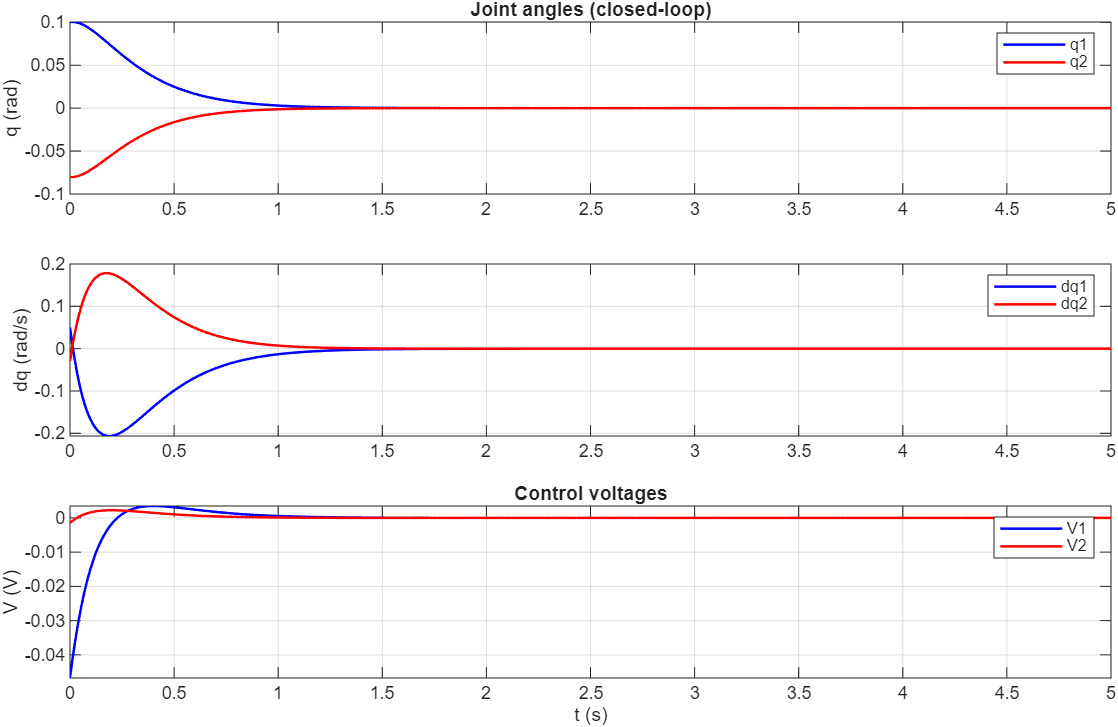
\includegraphics[width=\columnwidth]{page6_img1.jpeg}
\caption{Closed-loop equilibrium response: joint angles converge to zero (top), joint velocities decay (middle), and control voltages settle (bottom), confirming asymptotic stability.}
\label{fig:equilibrium}
\end{figure}

\section{Simulation Results}
\label{sec:simulation}

A complete non-linear simulation environment was implemented in MATLAB/Simulink with three operational modes managed by a Stateflow state machine (Fig.~\ref{fig:statemachine}): OFF, Position (POS), and Circle Trajectory (CIRCLE).

\begin{figure}[H]
\centering
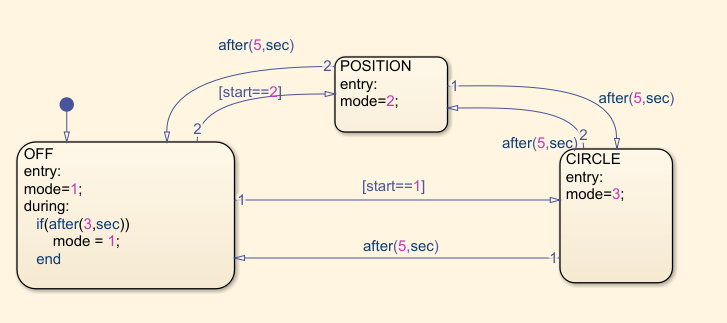
\includegraphics[width=0.85\columnwidth]{page13_img1.jpeg}
\caption{Stateflow state machine governing mode transitions: OFF $\to$ POSITION $\to$ CIRCLE, with timed transitions between states.}
\label{fig:statemachine}
\end{figure}

\subsection{Position Regulation}

The robot was commanded to move from $\mathbf{q}_{init} = [0, 0]$ to $\mathbf{q}_d = [0.5, 0.5]$\,rad. Two gain sets were compared:
\begin{itemize}
\item \textbf{Set~1} $(K_p, K_d) = (5, 1)$: Smooth convergence, overshoot $\sim$0.05\,rad, settling time $\sim$3\,s.
\item \textbf{Set~2} $(K_p, K_d) = (10, 3)$: Faster response, overshoot $\sim$0.01\,rad, settling time $\sim$1.5\,s.
\end{itemize}

Table~\ref{tab:gains} summarizes the trade-offs.

\begin{table}[H]
\centering
\caption{Effect of Gain Selection on System Response}
\label{tab:gains}
\begin{tabular}{lcc}
\toprule
\textbf{Characteristic} & \textbf{Low Gains} & \textbf{High Gains} \\
\midrule
Rise time & Slow & Fast \\
Overshoot & Higher & Lower \\
Settling time & Long & Short \\
Control effort & Low & High \\
Noise sensitivity & Low & High \\
Robustness & High & Moderate \\
\bottomrule
\end{tabular}
\end{table}

\subsection{Circular Trajectory Tracking}

The end-effector was commanded to trace a circle of radius $R = 0.3$\,m at $\omega = 0.5$\,rad/s. Fig.~\ref{fig:circle} shows the joint angle tracking performance: measured angles track desired references with phase error $< 0.02$\,rad and amplitude error $< 1\%$.

\begin{figure}[H]
\centering
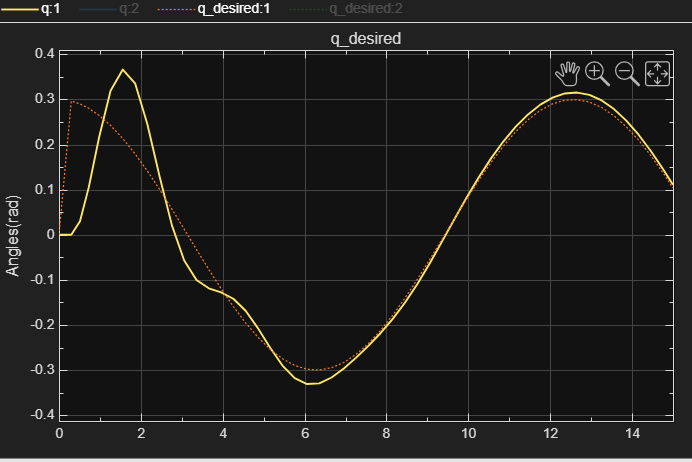
\includegraphics[width=\columnwidth]{page7_img1.jpeg}
\caption{Circular trajectory tracking: measured joint angles (solid) closely follow desired references (dashed) with minimal phase lag after initial transient.}
\label{fig:circle}
\end{figure}

\subsection{Hybrid Mode (Position $\to$ Trajectory)}

The full hybrid sequence (OFF $\to$ POS $\to$ CIRCLE) demonstrates seamless mode transitions (Fig.~\ref{fig:hybrid}): position regulation during 1--6\,s followed by smooth transition to circular tracking.

\begin{figure}[H]
\centering
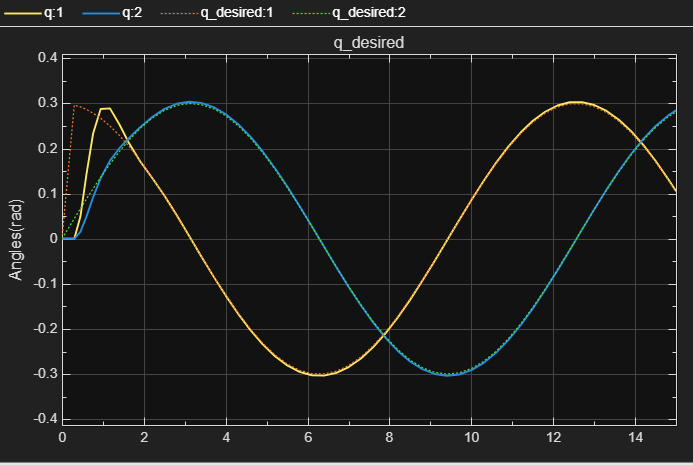
\includegraphics[width=\columnwidth]{page8_img1.jpeg}
\caption{Hybrid mode response showing sequential position regulation (1--6\,s) and circular trajectory tracking (6+\,s). The controller successfully manages mode transitions without destabilizing transients.}
\label{fig:hybrid}
\end{figure}

\section{Hardware Implementation}
\label{sec:hardware}

\subsection{Motor Selection}

The 25GA370 DC gear motor with integrated quadrature encoder (Fig.~\ref{fig:motor}) was selected for its favorable combination of torque capacity, encoder feedback, and direct voltage controllability. Table~\ref{tab:motor} summarizes its key specifications.

\begin{figure}[H]
\centering
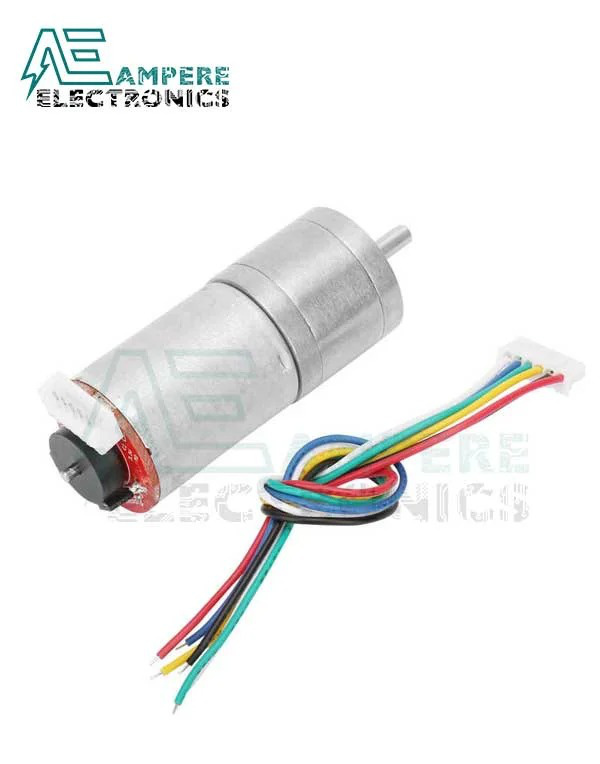
\includegraphics[width=0.6\columnwidth]{page10_img1.jpeg}
\caption{25GA370 DC gear motor with integrated quadrature encoder (Ampere Electronics). Six-wire interface provides motor power and encoder feedback~\cite{ampere2023}.}
\label{fig:motor}
\end{figure}

\begin{table}[H]
\centering
\caption{25GA370 Motor Specifications~\cite{ampere2023}}
\label{tab:motor}
\begin{tabular}{lcc}
\toprule
\textbf{Parameter} & \textbf{Value} & \textbf{Unit} \\
\midrule
Rated voltage & 12 & V DC \\
No-load speed & 200 & RPM \\
Rated power & 3 & W \\
Stall torque & 0.44 & N$\cdot$m \\
Gearbox ratio & 50:1 & -- \\
Encoder CPR (output) & 550 & counts/rev \\
\bottomrule
\end{tabular}
\end{table}

\subsection{Mechanical Design}

The mechanical structure was designed in SolidWorks (Fig.~\ref{fig:cad}) following the reference design by Benitez~\textit{et al.}~\cite{benitez2020}, with modifications for DC gear motors. Two rigid links were fabricated via 3D printing (PLA+) with custom couplers interfacing the 4\,mm D-type motor shafts to the link attachment points. The planar horizontal configuration eliminates gravitational torques.

\begin{figure}[H]
\centering
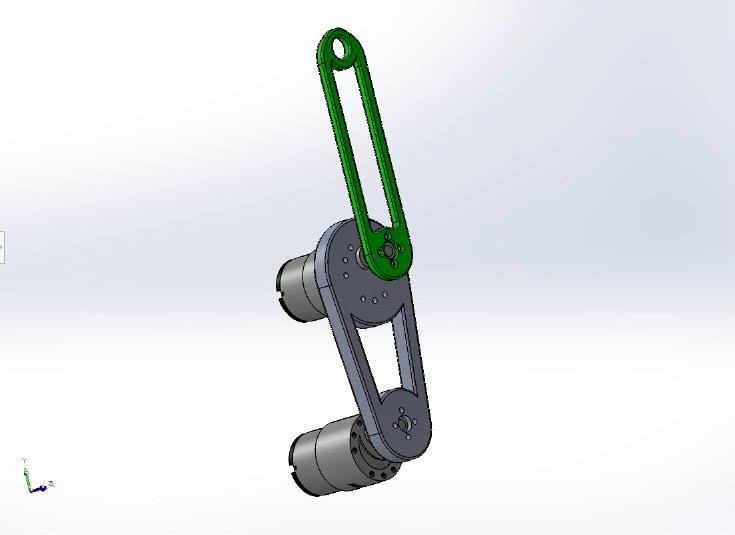
\includegraphics[width=0.7\columnwidth]{page11_img1.jpeg}
\caption{SolidWorks CAD assembly of the 2-DOF robotic arm showing both links (gray/green), motor housings at each joint, and mounting holes for hardware integration.}
\label{fig:cad}
\end{figure}

\subsection{Hardware Architecture}

The system uses an Arduino Mega 2560 for real-time control, an L298N dual H-bridge for bidirectional motor drive ($V_{supply}$ = 2.5--46\,V, 2\,A continuous per channel), and the integrated quadrature encoders (Fig.~\ref{fig:encoder}) for position feedback at 550 counts/revolution~\cite{mazeika2019}.

\begin{figure}[H]
\centering
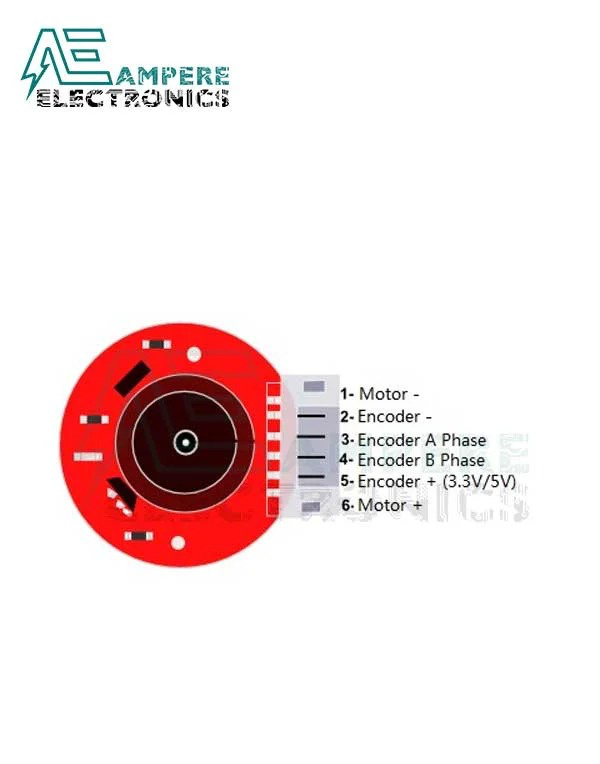
\includegraphics[width=0.6\columnwidth]{page12_img1.jpeg}
\caption{25GA370 encoder rear-view showing the 6-pin interface: Motor$\pm$, Encoder$\pm$ (3.3--5\,V), and quadrature channels A/B.}
\label{fig:encoder}
\end{figure}

The assembled prototype (Fig.~\ref{fig:prototype}) was verified through open-loop motor tests, encoder calibration (550 CPR confirmed), and closed-loop control execution before experimental testing.

\begin{figure}[H]
\centering
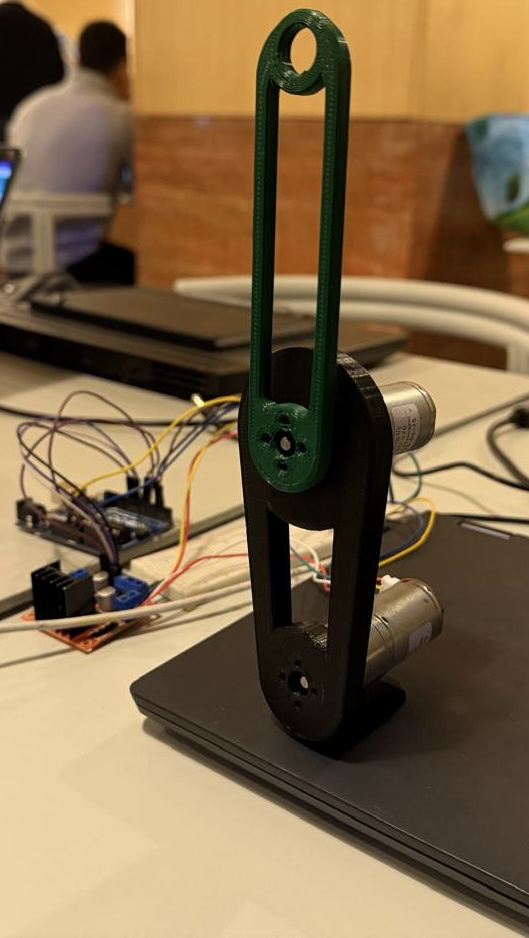
\includegraphics[width=0.65\columnwidth]{page12_img2.jpeg}
\caption{Fully assembled 2-DOF robotic arm prototype with 3D-printed links, DC gear motors, L298N driver, and Arduino controller, prepared for experimental testing.}
\label{fig:prototype}
\end{figure}

\subsection{Embedded Software}

The Arduino firmware implements a fixed-rate control loop ($T_s = 10$\,ms):
\begin{enumerate}
\item Read encoder counts, compute joint angles: $q = 2\pi \cdot \text{count} / 550$.
\item Estimate velocities via filtered finite differences: $\dot{q}_{filt}[k] = 0.7\dot{q}_{filt}[k{-}1] + 0.3\frac{\Delta q}{T_s}$.
\item Evaluate state machine (OFF/POS/CIRCLE) and generate references.
\item Execute feedback linearization: compute $\boldsymbol{\tau}_{des}$, convert to PWM voltages.
\item Apply saturation ($\pm$12\,V) and output to L298N.
\end{enumerate}

\section{Discussion}
\label{sec:discussion}

\subsection{Simulation Validation Summary}

The feedback linearization controller successfully:
\begin{itemize}
\item Decouples the non-linear joint dynamics as predicted by theory.
\item Achieves convergent position regulation ($< 0.01$\,rad steady-state error).
\item Tracks circular trajectories with $< 0.02$\,rad phase error.
\item Maintains bounded control effort within $\pm$12\,V actuator limits.
\end{itemize}

Lie-bracket controllability analysis confirmed rank$(V(\mathbf{x})) = 4$ across the entire workspace, verifying that no singular configurations exist.

\subsection{Hardware Discrepancy Sources}

Differences between simulation and hardware behavior arise from:
\begin{itemize}
\item Gearbox friction and backlash (not modeled).
\item Encoder quantization ($0.65^{\circ}$/count angular resolution).
\item PWM resolution limitations (8-bit, 256 levels).
\item Unmodeled structural compliance in 3D-printed links.
\end{itemize}

\subsection{Practical Recommendations}

\begin{enumerate}
\item Higher-resolution encoders would reduce velocity estimation noise significantly.
\item Friction compensation (Coulomb + viscous model) would improve low-speed tracking.
\item Adaptive control could handle parameter variations without explicit re-identification.
\end{enumerate}

\section{Conclusion}
\label{sec:conclusion}

This paper presented a complete non-linear control implementation for a 2-DOF planar robotic arm, spanning mathematical modeling, controller design, simulation validation, and hardware prototyping. Key achievements include:

\begin{enumerate}
\item Successful derivation and validation of the Euler--Lagrange dynamic model with DC motor electromechanical coupling.
\item Feedback linearization controller achieving convergent trajectory tracking with proven Lyapunov stability.
\item Demonstration of position regulation, circular trajectory tracking, and hybrid mode operation in MATLAB/Simulink.
\item Construction and verification of a physical prototype using commercially available components (25GA370 motors, L298N driver, Arduino Mega 2560).
\end{enumerate}

Future work includes friction compensation, adaptive control for parameter uncertainty, higher-resolution encoders, and extended workspace operation with obstacle avoidance.

\section*{Acknowledgment}

The authors thank Prof.\ Ayman A.\ El-Badawy and Eng.\ Karim Abdelsalam for their guidance and instruction throughout this project.

\begin{thebibliography}{7}

\bibitem{slotine1991}
J.~E. Slotine and W.~Li, \emph{Applied Nonlinear Control}.\hskip 1em plus 0.5em minus 0.4em Englewood Cliffs, NJ: Prentice-Hall, 1991.

\bibitem{spong2020}
M.~W. Spong, S.~Hutchinson, and M.~Vidyasagar, \emph{Robot Modeling and Control}, 2nd~ed.\hskip 1em plus 0.5em minus 0.4em New York: Wiley, 2020.

\bibitem{siciliano2009}
B.~Siciliano, L.~Sciavicco, L.~Villani, and G.~Oriolo, \emph{Robotics: Modelling, Planning and Control}.\hskip 1em plus 0.5em minus 0.4em Springer, 2009.

\bibitem{elbadawy2025}
A.~A. El-Badawy, ``Advanced mechatronics tutorial notes: Linearization, discretization, and feedback linearization,'' German University in Cairo, Course Material, 2025.

\bibitem{ampere2023}
Ampere Electronics, ``25GA370 DC gear motor with encoder specifications,'' 2023. [Online]. Available: https://ampere-electronics.com

\bibitem{benitez2020}
V.~H. Benitez, R.~Symonds, and D.~E. Elguezabal, ``Design of an affordable IoT open-source robot arm for online teaching of robotics courses during the pandemic contingency,'' \emph{HardwareX}, vol.~8, p.~e00158, 2020.

\bibitem{mazeika2019}
G.~Mazeika, ``H-bridge motor driver circuit,'' 2019. [Online]. Available: https://www.circuitjournal.com/h-bridge.html

\end{thebibliography}

\end{document}
